\documentclass{article}

\usepackage{caption}

\usepackage{multirow}

\usepackage{graphicx}
\setlength{\abovecaptionskip}{10pt plus 3pt minus 2pt}
\setlength{\belowcaptionskip}{10pt plus 3pt minus 2pt}

\usepackage[margin=1in]{geometry}

\usepackage{hyperref}
\hypersetup{
    pdfborderstyle={/S/U/W 1},
    colorlinks=true,
    linkcolor=blue,
    filecolor=magenta,
    urlcolor=cyan,
}

\usepackage{algorithm,algpseudocode}

\usepackage{xcolor}
\usepackage{listings}
\lstdefinestyle{DOS}{
    backgroundcolor=\color{lightgray},
    basicstyle=\scriptsize\color{black}\ttfamily
}

\title{
CSE 5441 (Fall 2019, Dr. Jones)\\
\large POSIX Threads AMR (Lab 2)
}
\author{
Caleb Lehman \\
\href{mailto:lehman.346@osu.edu}{lehman.346@osu.edu}
}

\begin{document}
\maketitle

\section*{Summary}
\label{sec:summary}

For this lab, I modified the previous serial \texttt{C} program to perform
Adapetive Mesh Refinement (AMR)\footnote{See previous lab or project
descriptions for details about AMR computation.} to work in parallel using the
POSIX Threads (\texttt{pthreads}) library. I created 4 programs,
\texttt{disposable}, \texttt{persistent}, \texttt{disposable\textunderscore equal\textunderscore boxes}, and
\texttt{persistent\textunderscore equal\textunderscore boxes}, which employ different strategies for 1)
thread creation and destruction and 2) distribution of boxes to threads. I
tested these programs on 3 test files with different numbers of threads to
compare performance against the serial version and against each other.
\label{subsec:results-summary}

As expected, the \emph{persistent threads} model outperformed the
\emph{disposable threads} model, most likely due to less overhead from not
destroying and recreating threads each iteration. All parallel programs
outperformed the serial version (at least for optimal choices of number of
threads).

\begin{itemize}

    \item The optimal number of threads for the smaller test case
    (\texttt{testgrid\textunderscore 400\textunderscore 12206}) was 6 for both
    programs.

    \item The optimal number of threads for the larger test case
    (\texttt{testgrid\textunderscore 1000\textunderscore 296793}) was $\sim$20
    for both programs.
    
    \item At the optimal numbers of threads, the \texttt{disposable} program
    was 1.9x faster than the serial program on the small test case and 9.2x
    faster on the large test case.

    \item At the optimal numbers of threads, the \texttt{persistent} program
    was 2.9x faster than the serial program on the small test case and 10.9x
    faster on the large test case.

    \item The different box-distribution strategies didn't make much of a
    difference, so I created a third test case, \texttt{testgrid\textunderscore
    512\textunderscore 196576} to emphasize disparities in the number of
    neighbors handled by each thread. Even in this case, there wasn't much
    difference (see the \hyperref[subsec:test_files]{Test Files} section for
    small discussion on this).

\end{itemize}

I used all 4 timing methods from lab 1 to collect timing data. All the timing
results I show in this report were collected from \texttt{clock\textunderscore
gettime}. Of particular note is that the \texttt{clock} function from the
\texttt{"time.h"} header is not particulary useful for our purposes, as it
reports CPU time, not wall time. As a result, it consistently returns a
significantly longer time than the actual time the program took to run.

\newpage
\section*{Pseudocodes}
\label{sec:pseudocoes}

This section contains rough pseudocodes for the (\texttt{*\textunderscore
equal\textunderscore boxes} versions of the) required programs. The pseudocode
for the main \texttt{disposable}/\texttt{persistent} programs is not listed,
but is equivalent except for the computation of $range$ being slightly more
involved in order to balance the number of neighbors handled by each thread.

\vspace{-1em}
\subsection*{\emph{Disposable Threads} Model}

Given $\alpha$, $\varepsilon$, a description of grid-aligned boxes, initial
Domain Specific Values (DSV), and a number of threads, the rough pseudocode for
my implementation following the \emph{disposable threads} model is as follows:

\begin{algorithm}
\small
\begin{algorithmic}[1]
\Procedure{Disposable}{$\alpha$, $\varepsilon$, $N$, $Boxes$, $Initial DSV$, $nthreads$}
\State $DSV \gets Initial DSV$, $DSV' \gets Initial DSV$
\While{$(\max{DSV} - \min{DSV})$ / $\max{DSV} > \varepsilon$} \label{alg:amr:convergence}
    \State Create $nthreads$ threads
    \ForAll{$threads$}
        \State \Call{Worker}{$\alpha$, $\varepsilon$, $N$, $Boxes$, $Initial DSV$, $nthreads$}
    \EndFor
    \State Join and destroy all threads
    \State $DSV \gets DSV'$ \label{alg:amr:commit}
\EndWhile
\EndProcedure
\Procedure{Worker}{$\alpha$, $\varepsilon$, $N$, $Boxes$, $Initial DSV$, $nthreads$}
    \State $tid \gets$ current thread number
    \ForAll{$i \in [ tid\cdot \frac{N}{nthreads}, (tid + 1)\cdot \frac{N}{nthreads} ]$}
        \State $DSV'[i] \gets (1 - \alpha)\cdot DSV[i] + \alpha \cdot \sum_{j\in nhbr} DSV[j]\cdot \Call{Overlap}{i, j, Boxes}$
    \EndFor
\EndProcedure
\end{algorithmic}
\end{algorithm}

To summarize, under this model, threads are created at the beginning of each
iteration and execute updates in parallel. Then the threads are joined and
destroyed and the updates are committed.

\vspace{-1em}
\subsection*{\emph{Persistent Threads} Model}

Given $\alpha$, $\varepsilon$, a description of grid-aligned boxes, initial
Domain Specific Values (DSV), and a number of threads, the rough pseudocode for
my implementation following the \emph{persistent threads} model is as follows:

\begin{algorithm}
\small
\begin{algorithmic}[1]
\Procedure{Persistent}{$\alpha$, $\varepsilon$, $N$, $Boxes$, $Initial DSV$, $nthreads$}
\State $DSV \gets Initial DSV$, $DSV' \gets Initial DSV$
\State Create $nthreads$ threads to execute \Call{Worker}{$\alpha$, $\varepsilon$, $N$, $Boxes$, $DSV$, $DSV'$, $nthreads$}
\State Join and destroy all threads
\EndProcedure
\Procedure{Worker}{$\alpha$, $\varepsilon$, $N$, $Boxes$, $DSV$, $DSV'$, $nthreads$}
    \State $tid \gets$ current thread number
    \State $range \gets [ tid\cdot \frac{N}{nthreads}, (tid + 1)\cdot \frac{N}{nthreads} ]$
    \While{$(\max{DSV} - \min{DSV})$ / $\max{DSV} > \varepsilon$}
        \ForAll{$i \in range$}
            \State $DSV'[i] \gets (1 - \alpha)\cdot DSV[i] + \alpha \cdot \sum_{j\in nhbr} DSV[j]\cdot \Call{Overlap}{i, j, Boxes}$
        \EndFor
        \State \texttt{BARRIER} to sync all threads
        \State $DSV[range] \gets DSV'[range]$
        \State \texttt{BARRIER} to sync all threads
    \EndWhile
\EndProcedure
\end{algorithmic}
\end{algorithm}

To summarize, under this model, threads are created at the beginning of the
program and destroyed at the end. The threads run in parallel, updating each of
their blocks of DSVs. The threads are synchronized twice per iteration: 1)
after computing the updates and 2) after commiting updates.

\section*{Tests}
\label{sec:tests}

\subsection*{Environment}
\label{subsec:environment}

The program was developed and tested on a single, 40-core node of the
\href{https://www.osc.edu/resources/technical_support/supercomputers/pitzer}{Pitzer
cluster} at the \href{https://www.osc.edu/}{Ohio Supercomputer Center}.

For development, I loaded the \texttt{intel/18.0.3} module, which allowed the
program to be compiled with version 18.0.3 of the \texttt{icc} C-compiler. I
linked against the \texttt{librt} and \texttt{libpthread} libraries.

For testing, I loaded the \texttt{python/3.6-conda5.2} module, which loads a
python environment with the \texttt{NumPy}, \texttt{SciPy}, and
\texttt{Matplotlib} packages, among others.

\subsection*{Timing}
\label{subsec:timing}

I collected timing data using the same 4 methods as the first lab:
\texttt{time}, \texttt{clock}, and \texttt{clock\textunderscore gettime} from
the \texttt{"time.h"} header; and the \texttt{UNIX} utility \texttt{time}.

I didn't use the results from the \texttt{clock} function from the
\texttt{"time.h"} header, since it reports CPU time, not wall time. The other
methods all returned values within 1 second of each other. The \texttt{time}
function declared in \texttt{"time.h"} returns an integer number of seconds,
but the other two methods return with sub-second precision.  \emph{For
consistency, I used the \texttt{clock\textunderscore gettime} function for all
results in this report}.

\subsection*{Test Files}
\label{subsec:test_files}

Dr. Jones provided the \texttt{testgrid\textunderscore 400\textunderscore
12206} test file.  As part of lab 1, I reduced the $\alpha$ (affect rate) and
$\varepsilon$ parameters until the serial runtime increased into the 3 to 6
minute range. In particular, I selected $\alpha = 0.01$ and $\varepsilon =
0.02$, for which the serial program completed in 261 seconds.

The above approach of changing the $\alpha$ and $\epsilon$ parameters allows us
to make the programs run longer, but doesn't affect the actual length of each
iteration. With only 12206 boxes, each iteration is fairly short (on the order
of $\frac{261\textrm{ sec}}{1589637} = 0.16\textrm{ms}$ per iteration), so it is
expected the overhead of synchronizing threads would inhibit parallelizing
beyond a small number of threads. In order to investigate this, I generated
another test file, \texttt{testgrid\textunderscore 1000\textunderscore 296793},
which has more boxes and therefore longer iterations.

As mentioned above, in addition to the two required programs, I created two
more with different distibutions of boxes to threads. I expected the programs
which balanced the number of neighbors for which each thread was responsible
(\texttt{disposable} and \texttt{persistent}) to outperform the programs which
simply gave equally-sized, contiguous chunks of boxes to each thread the number
of boxes (\texttt{*\textunderscore equal\textunderscore boxes}), since number of neighbors controls how much
``work'' is done for each box. However, both programs performed similarly on
the first two test files. I created a third test file
\texttt{testgrid\textunderscore 512\textunderscore 196576}, in which
different are areas of the grid have different average neighbors per box. Even on
this specialized test case, there was no non-trivial performance difference.
Reflecting on this comparison, I think attempting to optimize the number of
neighbors handled by each thread is not too promising, since the overall
average number of neighbors per box in a grid (actually for any planar graph)
is always strictly $<6$, so the typical grid is not pathalogical enough for it
to make a difference.

Some summary statistics for the test files are presented below. Per submission
instructions, I didn't include the test files with the code submission, but I
can produce them if needed.

\begin{table}[b]
    \centering
    \begin{tabular}{|c|c|c|c|c|c|}
        \hline
        test & \texttt{\#} rows & \texttt{\#} cols & \texttt{\#} boxes & mean \texttt{\#} neighbors & std. dev. \texttt{\#} neighbors \\
        \hline
        \hline
        \texttt{testgrid\textunderscore 400\textunderscore 12206} & 400 & 400 & 12206 & 5.89 & 1.55 \\
        \texttt{testgrid\textunderscore 1000\textunderscore 296793} & 1000 & 1000 & 296793 & 4.79 & 1.57 \\
        \texttt{testgrid\textunderscore 512\textunderscore 196576} & 512 & 640 & 196576 & 5.32 & 18.24 \\
        \hline
    \end{tabular}
    
    \caption{Basic statistics for my test files. Note that the file in the
    second row was engineered to have many boxes and the file in the third row
    was engineered to have high variance/std. dev.}

\end{table}

\newpage
\section*{Results}
\label{sec:results}

The output for each test case was consistent across all variations and was as follows:
\begin{itemize}
    \item \texttt{testgrid\textunderscore 400\textunderscore 12206}: 1589637 iterations, $(max, min) = (0.085900, 0.084182)$
    \item \texttt{testgrid\textunderscore 1000\textunderscore 296793}: 51684 iterations, $(max, min) = (0.000000, 0.000000)$
    \item \texttt{testgrid\textunderscore 512\textunderscore 196576}: 63380 iterations, $(max, min) = (0.000000, 0.000000)$
\end{itemize}

The main timing results are shown in the figure below. I ran the programs for
various amounts of threads between 1 and 40. Note that for the provided test
file \texttt{testgrid\textunderscore 400\textunderscore 12206}, the optimal
number of threads was around 6 for each program, while the optimal number of
threads was around 20 for the larger test files that I created. This confirms
that increasing the number of boxes, thereby increasing the (serial) length of
each iteration provides more opportunities for parallelism. The iterations for
the small test file are so short that the overheads associated with
creating/destroying/synchronizing threads quickly becomes the bottleneck.

Other notes are that \texttt{persistent} versions consistently outperformed
\texttt{disposable} versions, as expected, and that my variations with how
boxes were distributed had very little effect. Finally, the parallel versions
of the program did outperform the serial version, except for the smallest test
case, where, for large number of threads, the overheads outweighed the benefits
of parallelism and the parallel programs actually performed worse.

\vspace{3em}
\begin{minipage}{\linewidth}
    \centering
    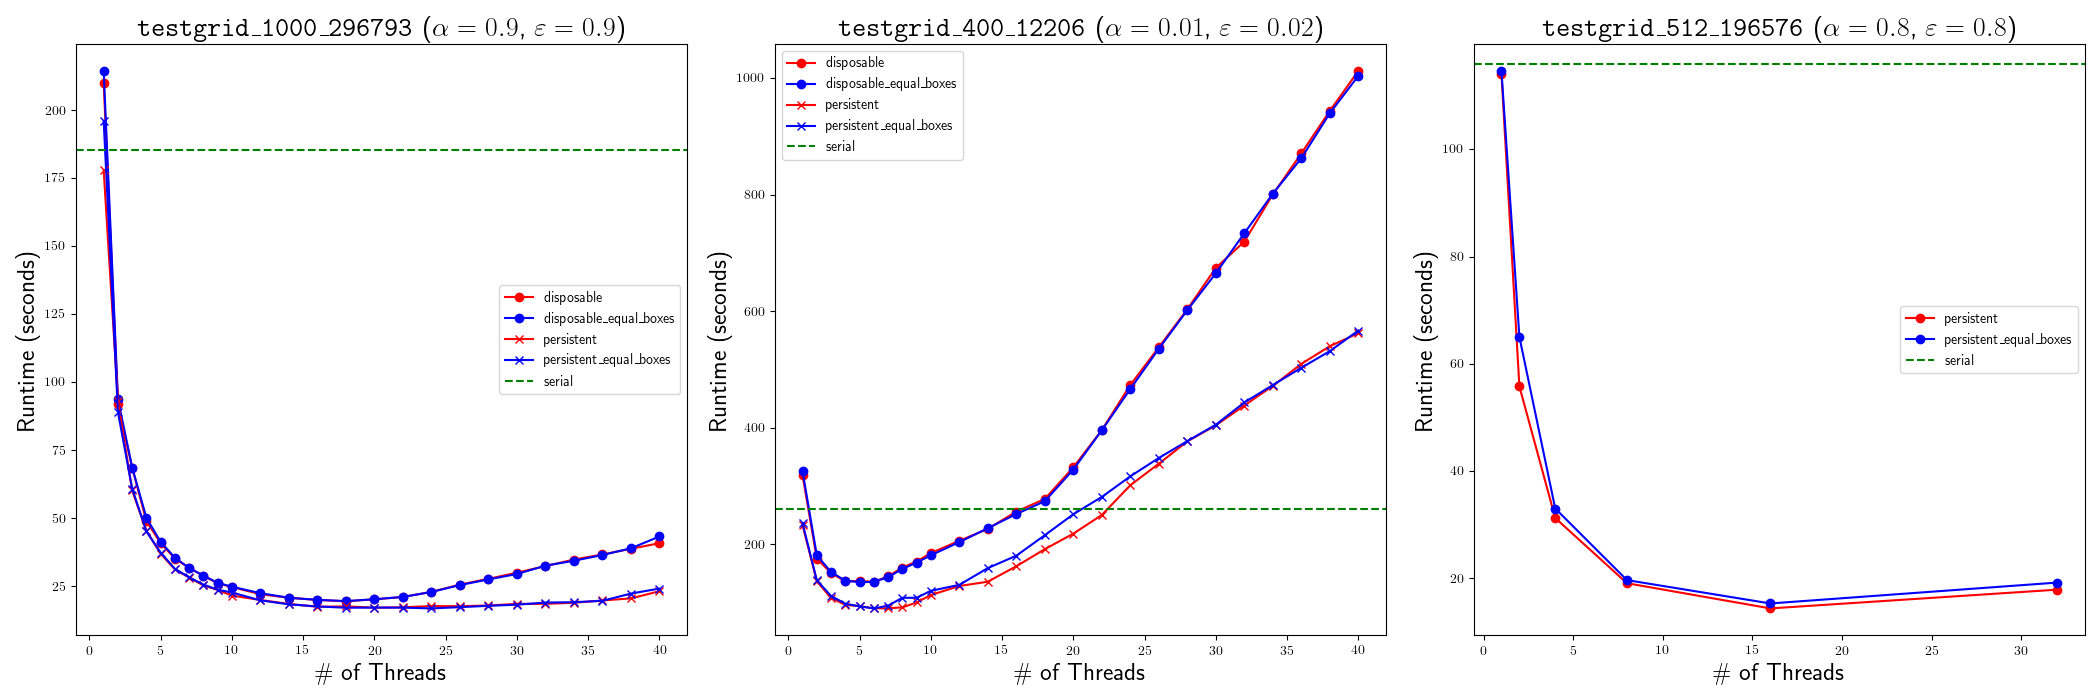
\includegraphics[width=\linewidth]{../results/plot.png}

    \captionof{figure}{The runtimes of the parallel versions of the program
    plotted against the number of threads used. Serial runtime is included for
    comparison. Note that \texttt{persistent} consistently outperforms
    \texttt{disposable} and that the \texttt{*\textunderscore
    equal\textunderscore boxes} versions perform similarly to their
    counterparts. Also note that \texttt{persistent} switches from \texttt{x}
    markers to circle markers in the rightmost plot.}

    \label{fig:runtimes}
\end{minipage}

\newpage
\section*{Project Usage}
\label{sec:project}

\subsection*{Building}
\label{subsec:building}

To build the required \texttt{disposable} and \texttt{persistent} executables
(as well as the \texttt{*\textunderscore equal\textunderscore boxes}) variations, navigate to the top level
of the submitted directory and build as follows:

\begin{lstlisting}[style=DOS]
# Ensure that you have icc compiler

$ make
...
$ ls
... disposable disposable_equal_boxes persistent persistent_equal_boxes ...
\end{lstlisting}

\subsection*{Running}
\label{subsec:running}

The syntax to run the program is:

\begin{lstlisting}[style=DOS]
$ ./[program] [affect-rate] [epsilon] [num-threads] <[test-file]
\end{lstlisting}

where \texttt{program} is one of the built programs and \texttt{num-threads} is
any positive integer number of threads.

\end{document}
